\chapter{Experimental Setup of a Small Angle Scattering Instrument}
\section{SANS-Camera}
\begin{figure}[htb]
\begin{center}
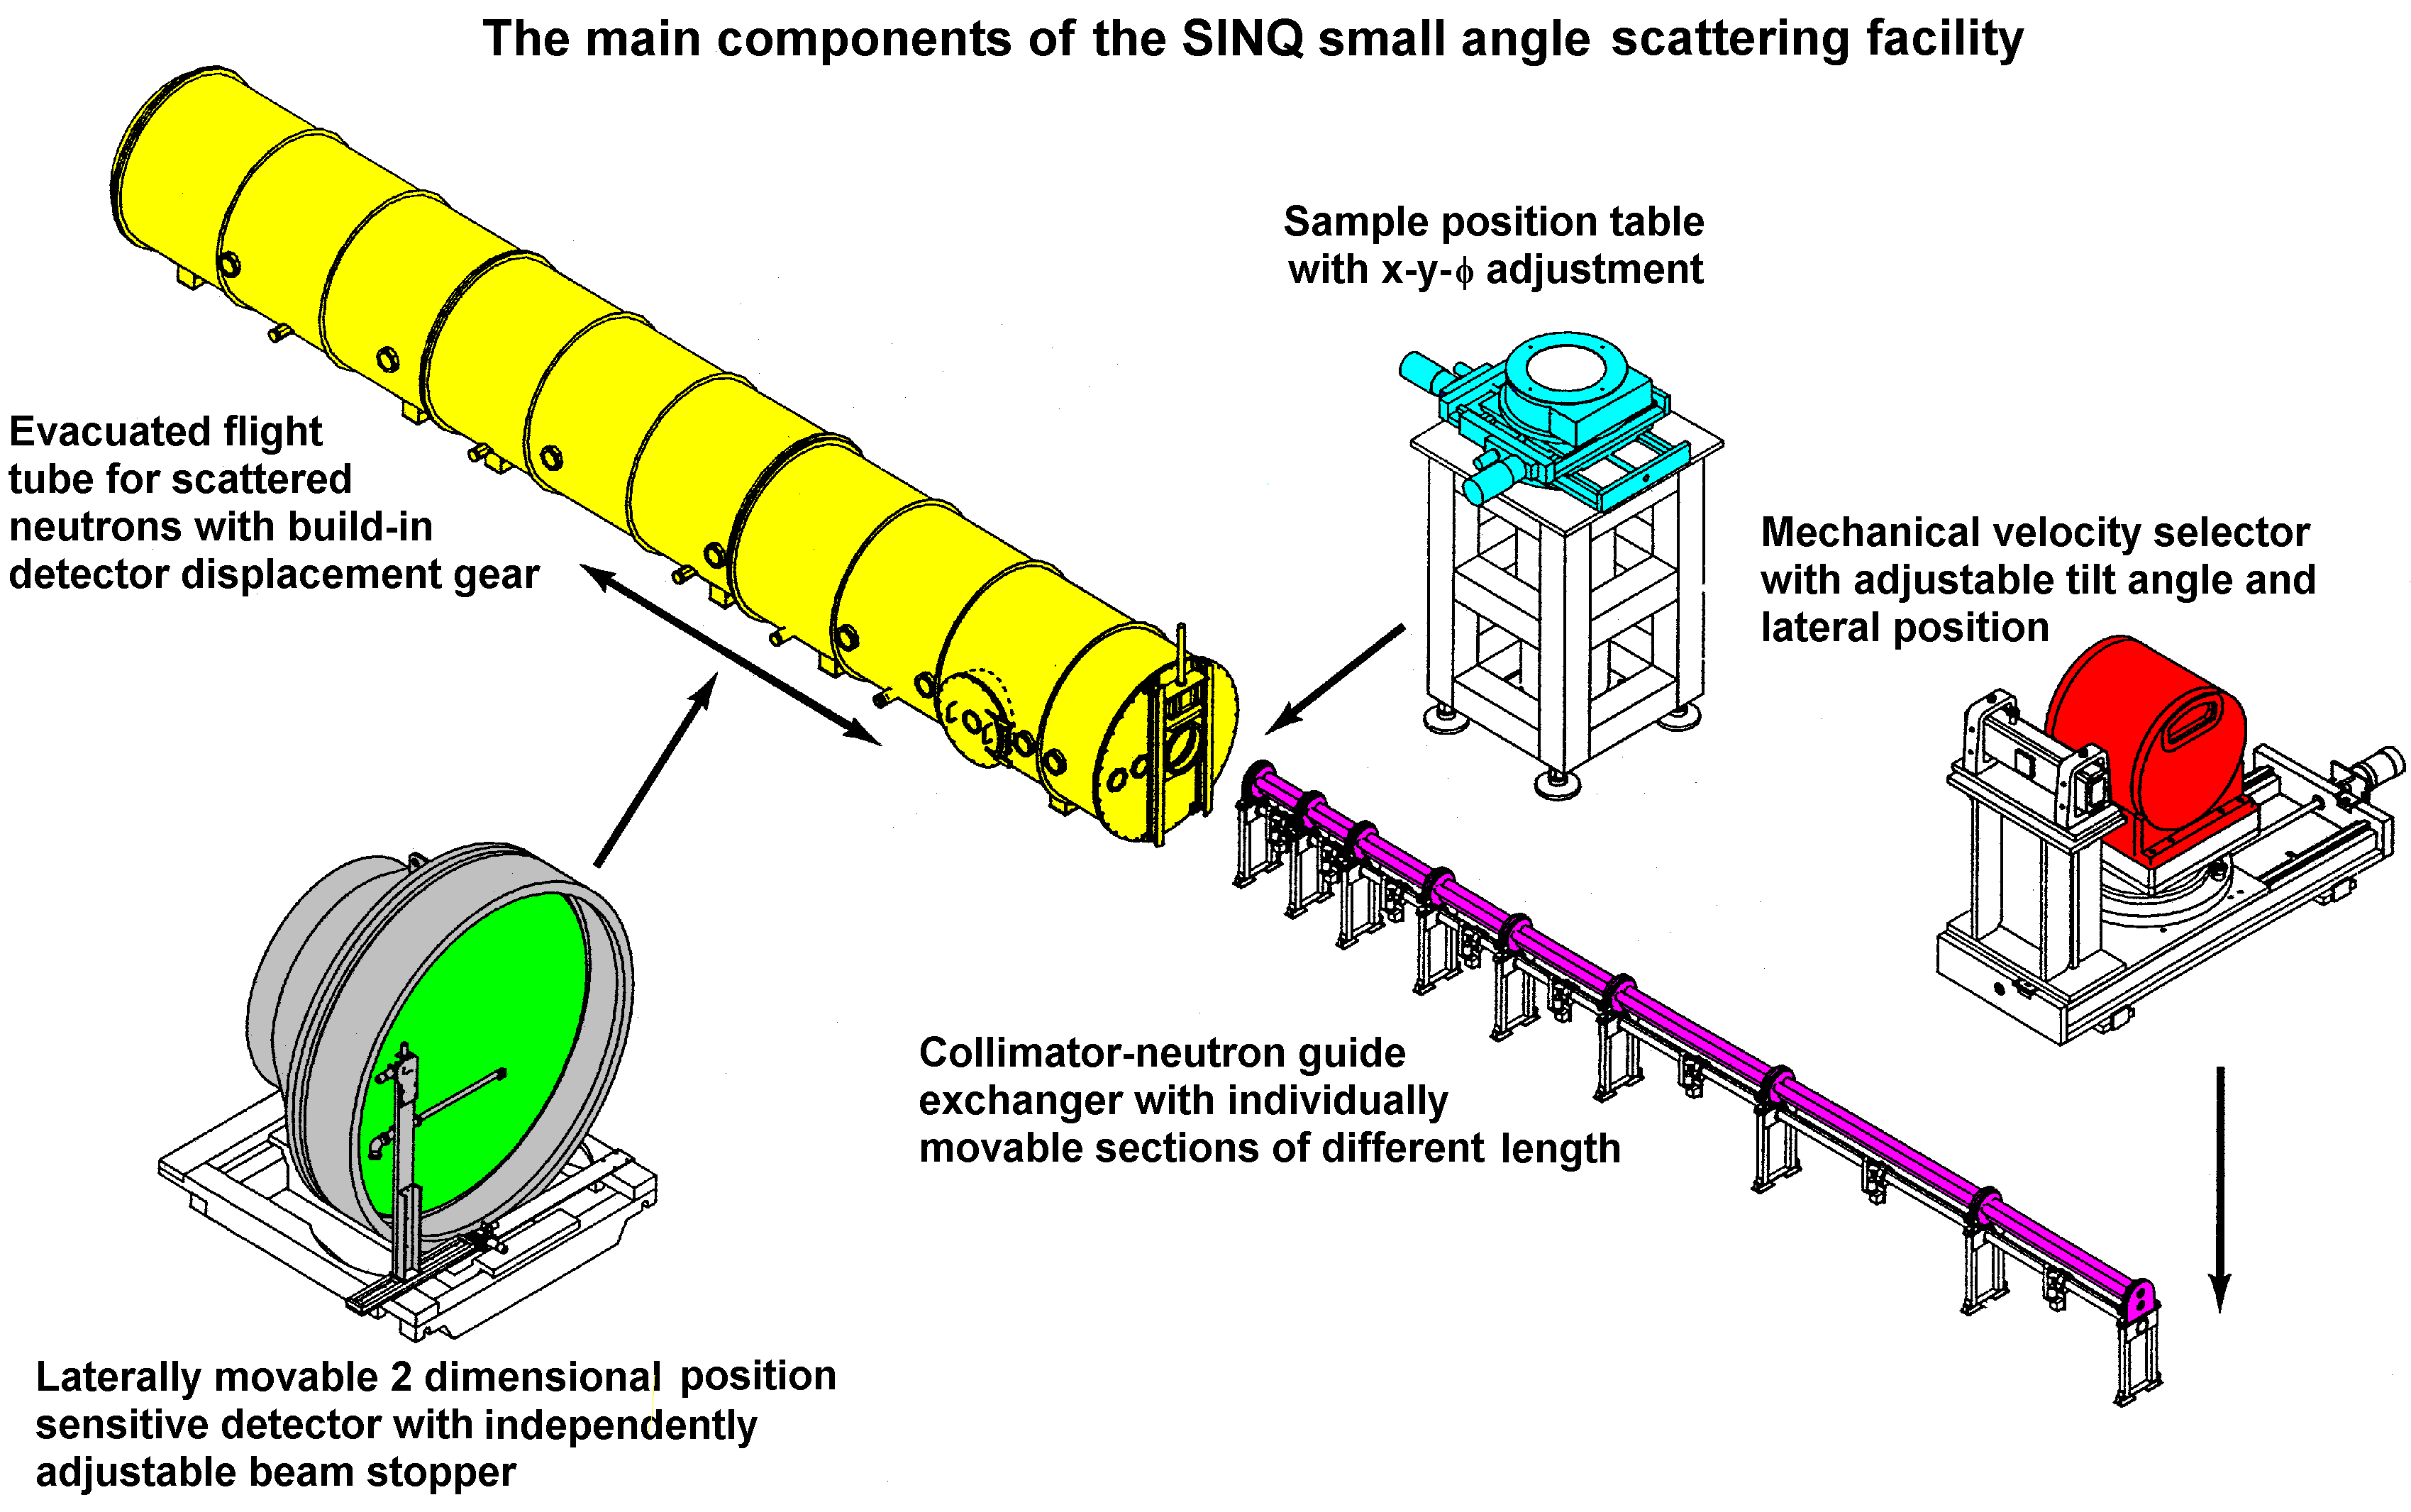
\includegraphics[width=\textwidth,height=0.627\textwidth]{SANSAN.png}
\caption{SANS-1 instrument at PSI, Switzerkand} \label{SANS1@PSI}
\end{center}
\end{figure}

\section{SAXS-Camera}

\begin{figure}[htb]
\begin{center}
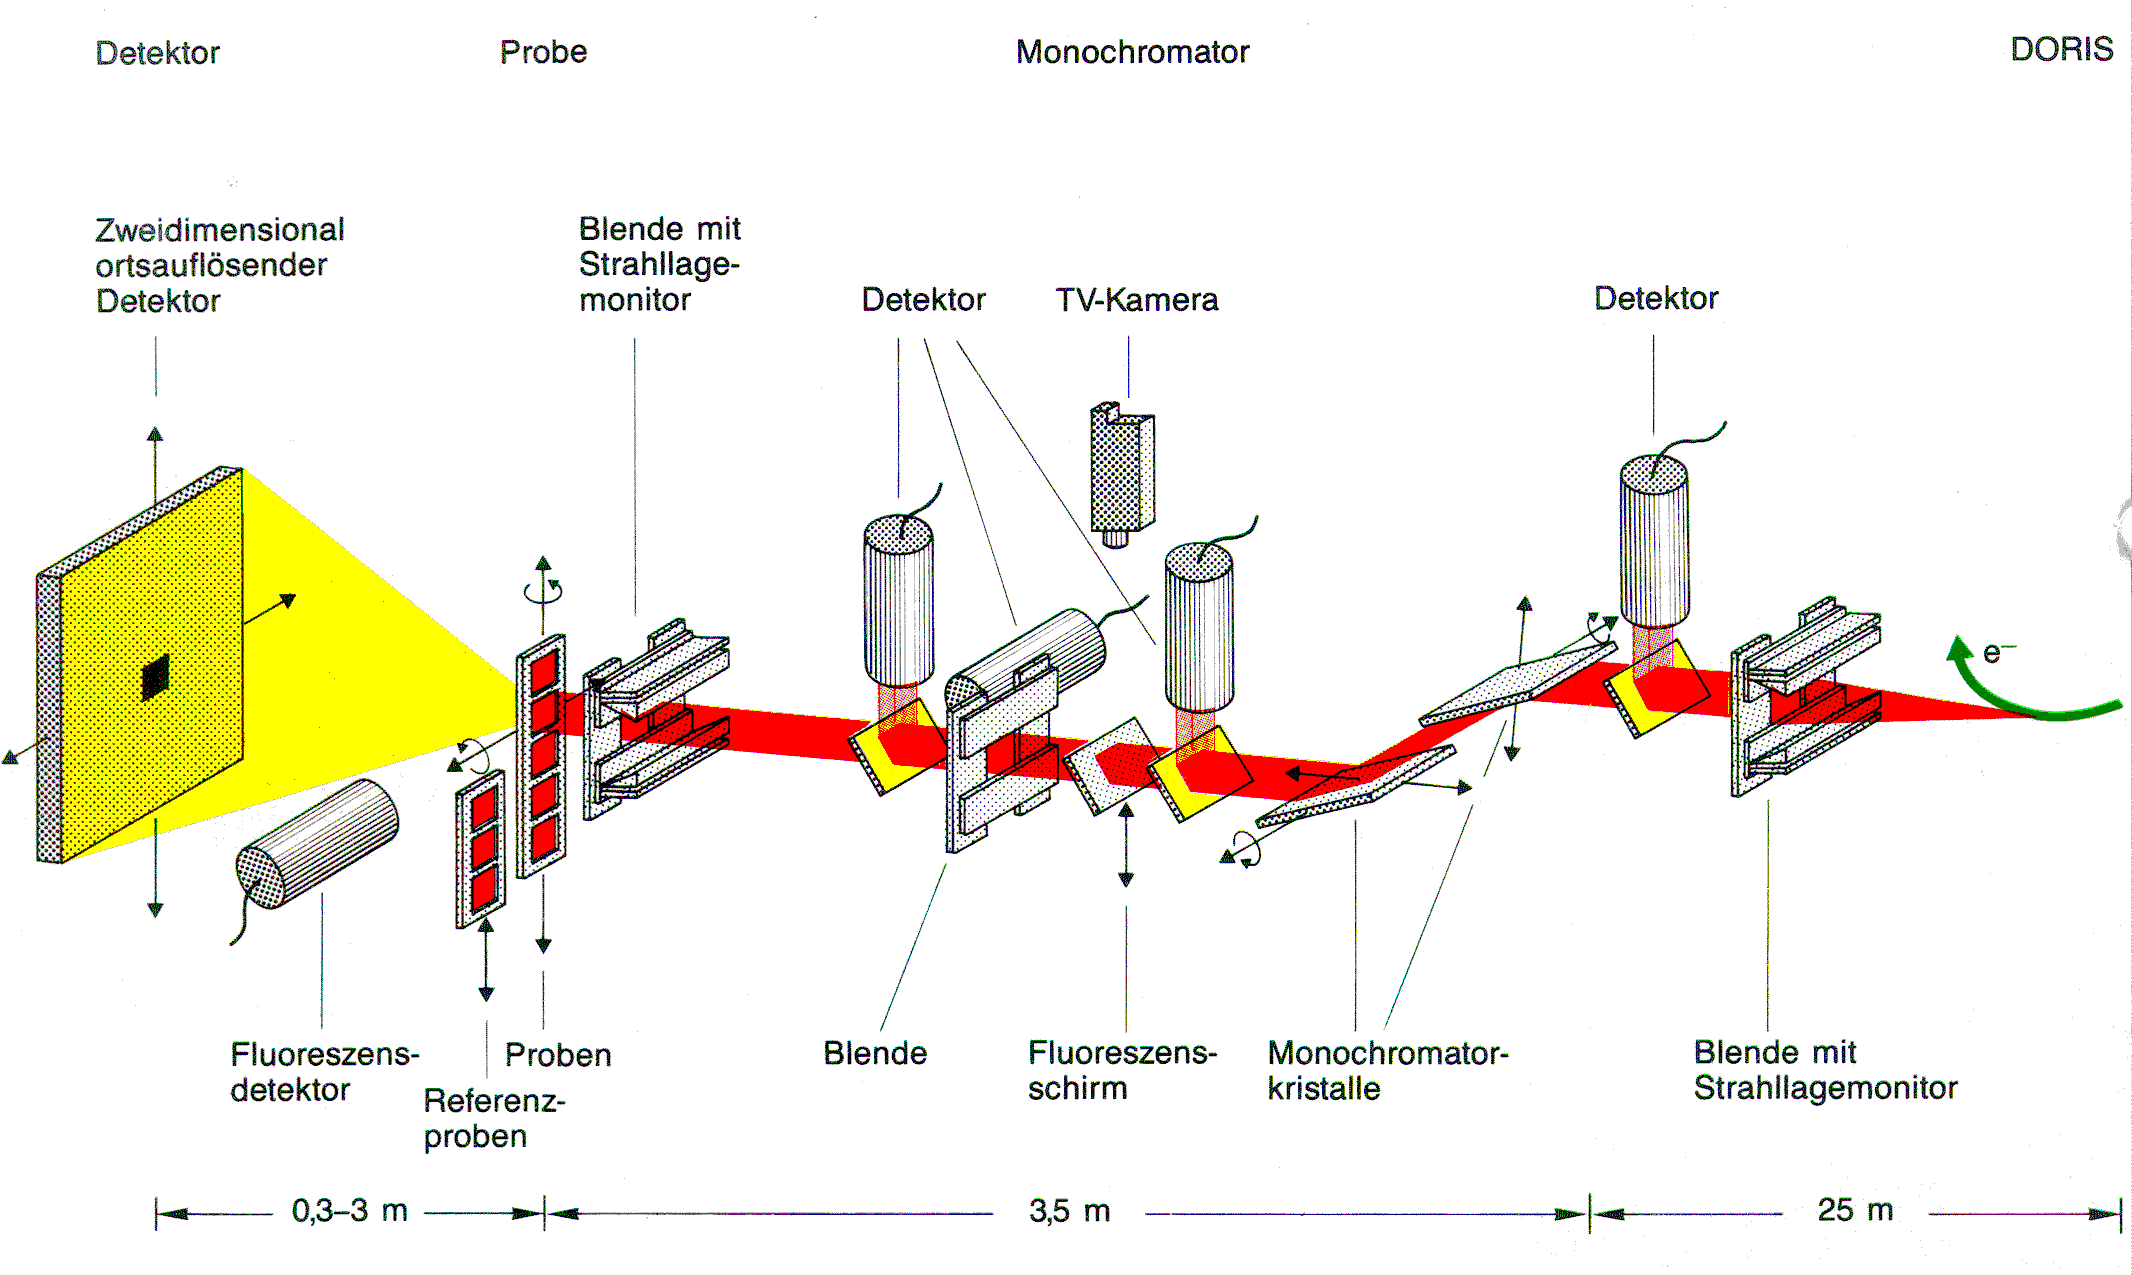
\includegraphics[width=\textwidth,height=0.598\textwidth]{CJUSIFA.png}
\caption{Small angle x-ray scattering instrument Jusifa at the
synchrotron light source HASYLAB in Hamburg} \label{Jusifa}
\end{center}
\end{figure}

\chapter{Data Reduction in SAS}

\section{Correction and Normalization of SANS-Raw data}

A detector of a small angle scattering camera measures the
superposition of intensities of different origin:
\begin{enumerate}
\item Background noise $I_B$
\item Scattering of the empty sample holder $I_{H}$
\item scattering of the isolated sample $I_S$
\end{enumerate}
Furthermore the detector elements can have different efficiencies $\epsilon_i$.
To determine the differential cross-section of of the sample all the different
contribution to the total scattering intensity have to be considered and determined
separately by different measurements. The quantity to be known is the scattering
contribution of the isolated sample $I_S$, which in general can not be measured directly.
Experimental accessible scattering contributions are the scattering of the sample in the
sample holder $I_{S+H}$, the contribution of the empty sample holder $I_{H}$ and the
background noise $I_B$. From this experimental accessible data the wanted scattering
contribution of the isolated sample has to be determined.

\subsection{Contribution of the isolated sample}
The intensity of the incident beam will be attenuated by absorption
and scattering effects within the sample. Also the scattered neutrons
will be further attenuated on their residual path through the sample.
The measured intensity in a detector element  $i$ is given by
\begin{equation}
I^0_{S,i} = \int^d_0 dx\, \Phi_0\, \Delta \Omega_i\, \epsilon_i\,
e^{-\alpha\,x}\, A\, \rho \, e^{-\frac{\alpha(d-x)}{\cos\theta}}
\left\{ \frac{d\sigma_{\rm coh}}{d\Omega} + \frac{d\sigma_{\rm inc}}{d\Omega}
\right\}
.
\end{equation}
Hereby $d$ describes the sample thickness in cm, $\Phi_0$ the incident neutron
flux in neutrons per cm$^2\times$sec, $d\Omega_i$ is the solid angle of the detector
element $i$ in steradian, $\epsilon_i$ the detection efficiency of detector element
$i$ and $\alpha$ the extinction coefficient of the sample in cm$^{-1}$. $A$ the illuminated
sample area in cm$^2$. $\theta$ describes the angle between the wave vector  ${\bf k}_0$ of
the incident neutrons and the wave vector ${\bf k}$ of the scattered neutrons.
$\frac{d\sigma_{\rm coh}}{d\Omega}$ and
$\frac{d\sigma_{\rm inc}}{d\Omega}$ are the coherent and incoherent differential cross-sections,
respectively.
For small angle scattering $\cos\theta \simeq 1$ and one yields after integration
\begin{equation}
I^0_{S,i} = \Phi_0\, \Delta \Omega_i\, \epsilon_i\,
\underbrace{A\, \rho \,d}_{N_S}\, \underbrace{e^{-\alpha d}}_{T_S}
\left\{ \frac{d\sigma_{\rm coh}}{d\Omega} + \frac{d\sigma_{inc}}{d\Omega}
\right\}
.
\end{equation}
The quantity $N_S = A\, \rho\, d$ corresponds to the number of scattering
atoms and $T_S = e^{-\alpha\, d} = \frac{I_{\rm trans}}{I_0}$ to the transmissions
coefficient, which can be determined from the ration of the intensity of the
transmitted primary beam $I_{\rm trans}$ and the intensity of the incident beam
$I_0$. The incoherent scattering is isotropically and equally distributed over
the whole solid angle of  $4\pi$. Therefore one gets for $I^0_{S,i}$
\begin{equation}
I^0_{S,i} = \Phi_0\, \Delta \Omega_i\, \epsilon_i\,
\left\{ N_S\, T_S \, \frac{d\sigma_{\rm coh}}{d\Omega} + A\, \frac{1-T_S}{4\,
\pi} \right\} . \label{dsdotheo}
\end{equation}

\subsection{Correction for sample holder and background noise}
The scattering intensity of an isolated sample can practically never
measured directly. The scattering of the sample is always superposed
by scattering from the sample holder and by background noise. Background noise
is meant to be electronic noise, cosmic radiation, and detection of neutrons, which
have not passed through the sample like scattered neutrons from neighboring experiments.
Because of this reasons additional measurements have to be carried out, which are
a measurement of the empty sample holder $I_H$ and a measurement with a strong
absorber like Cadmium in front of the sample to measure the background noise $I_B$.
Together with the measurement of the sample in the sample holder $I_{S+H,i}$
 the scattering of the isolated sample $I^0_{S,i}$ on the detector element $i$ can
 be calculated by
\begin{equation}
I_{S,i}^0 = \left( \frac{I_{S+H,i}}{M_{S+H}} - \frac{I_{B,i}}{M_B} \right)
-
\frac{T_{S+H}}{T_H} \left(\frac{I_{H,i}}{M_{H}} - \frac{I_{B,i}}{M_B} \right) .
\label{dsdoexp}
\end{equation}
The index $B$ stands for \underline{b}ackground, $H$
for the empty sample \underline{h}older, $S+H$ for the sample in the sample holder and $S$
for the scattering of the isolated sample.
All intensities have to be normalized on the number of incident neutrons. This can be done
for example by division of the measured intensity my a monitor count rate $M$.
The factor $ \frac{T_{S+H}}{T_H}$ takes account for the attenuation of the beam by the sample.

The differential cross-section in eq.\ \ref{dsdotheo} can now be calculated from the measurable
intensities in eq.\ \ref{dsdoexp}. Nevertheless the quantities $\Phi_0$, $\Delta\Omega_i$ and
$\epsilon_i$ still have to be known. Furthermore $I_S^0$ is not given in physical standard units
but in units per monitor count. All this can be overcome by a comparison with a standard substance
$St$. Common standard materials are in general materials with a small coherent cross-section and a
large incoherent cross-section like vanadium or water. For both of these materials the coherent
cross-section is negligible small. The scattering intensities of the standard materials have to be
corrected in the same way than the sample itself according to eq.\ \ref{dsdoexp}. The ratio of both
intensities $I^0_{S,i}/I^0_{St,i}$ leads to
\begin{equation}
\frac{I^0_{S,i}}{I^0_{St,i}} = \frac{T_S\, N_S\, \displaystyle
\left(\frac{d\sigma_{\rm coh}}{d \Omega} +
\frac{d\sigma_{\rm inc}}{d\Omega} \right)}{T_{St}\,N_{St}\, \displaystyle
\frac{d\sigma^{St}_{\rm inc}}{d\Omega}}
\end{equation}
\begin{equation}
\Leftrightarrow \qquad \displaystyle
\frac{d\sigma_{\rm coh}}{d\Omega} + \frac{d\sigma_{\rm inc}}{d\Omega} =
\frac{I^0_{S,i}}{I^0_{St,i}} \, \frac{T_{St}\, N_{St}}{T_S\, N_S}\,
\displaystyle
\frac{d\sigma^{St}_{\rm inc}}{d\Omega}
\end{equation}
\begin{equation} \displaystyle
\mbox{or}\qquad
\frac{d\sigma_{\rm coh}}{d\Omega} + \frac{d\sigma_{\rm inc}}{d\Omega} =
\frac{I^0_{S,i}}{I^0_{St,i}} \, \frac{(1-T_{St})\, \displaystyle
\frac{A_{St}}{4\pi}}{T_S\, N_S} .
\end{equation}
If water is used as a standard the last formula has to be multiplied on the right
side with an empirical factor $f(\lambda,\sigma_t,T) \simeq 1$. This factor corrects for
the different efficiencies of the detector for different neutron energies. This correction
can become important in case of water because of it inelastic scattering behavior.

\section{Correction and normalization of SAXS raw data}
